% Necoyoad Architecture Blueprint v7 — Menu Links in Admin and Apps
\documentclass[11pt,a4paper]{article}
\usepackage[T1]{fontenc}
\usepackage[utf8]{inputenc}
\usepackage{lmodern}
\usepackage{microtype}
\usepackage{graphicx}
\usepackage{xcolor}
\usepackage{geometry}
\usepackage{amsmath}
\usepackage{amssymb}
\usepackage{tcolorbox}
\tcbuselibrary{skins,breakable,listings}
\usepackage{colortbl}
\usepackage{booktabs}
\usepackage{tabularx}
\usepackage{longtable}
\usepackage{array}
\usepackage{enumitem}
\usepackage{adjustbox}
\usepackage{caption}
\usepackage{fancyhdr}
\usepackage{titlesec}
\usepackage{pdflscape}
\usepackage{listings}
\usepackage{tikz}
\usetikzlibrary{arrows.meta,positioning,calc,shapes.geometric,fit,backgrounds,chains,decorations.pathreplacing,shapes.multipart}
\usepackage[colorlinks=true,linkcolor=blue!50!black,citecolor=blue!40!black,urlcolor=blue!60!black,bookmarks=true,bookmarksnumbered=true,unicode=true,pdftitle={Necoyoad - Menu Links in Admin and Apps (v7)},pdfauthor={Reverse-Engineered Architecture Report},pdfsubject={Software Architecture, Menu System, Navigation, Widget Rendering},pdfkeywords={Necoyoad, OpenCart, PHP 8.1, Menu, Menu Link, Navigation, Links Widget, Tree, EAV Property}]{hyperref}
\geometry{a4paper, top=2.4cm, bottom=2.4cm, left=2.4cm, right=2.4cm}
\setlength{\headheight}{14pt}
\pagestyle{fancy}
\fancyhf{}
\fancyhead[L]{\small\itshape Necoyoad v7 --- Menu Links in Admin and Apps}
\fancyfoot[C]{\small\thepage}
\renewcommand{\headrulewidth}{0.3pt}
\renewcommand{\footrulewidth}{0pt}
\titleformat{\section}{\Large\bfseries\color{black!85}}{\thesection}{0.6em}{}
\titleformat{\subsection}{\large\bfseries\color{black!80}}{\thesubsection}{0.6em}{}
\titleformat{\subsubsection}{\normalsize\bfseries\color{black!75}}{\thesubsubsection}{0.5em}{}
\widowpenalty=10000
\clubpenalty=10000
\emergencystretch=4em
\hbadness=10000
\hfuzz=2pt
\vfuzz=2pt
\sloppy
\definecolor{necoyoad-blue}{HTML}{1F4E79}
\definecolor{necoyoad-orange}{HTML}{B85C00}
\definecolor{necoyoad-green}{HTML}{2E6B33}
\definecolor{nodefill}{HTML}{F4F7FB}
\definecolor{nodefillalt}{HTML}{FBF4EE}
\definecolor{nodefillgreen}{HTML}{F2F8F2}
\definecolor{nodefillgray}{HTML}{F0F0F2}
\definecolor{phpline}{HTML}{F8F8F0}
\definecolor{phpcomment}{HTML}{8C8C8C}
\definecolor{phpkeyword}{HTML}{1F4E79}
\definecolor{phpstring}{HTML}{B85C00}
\lstdefinelanguage{necophp}{
  morekeywords={abstract,and,array,as,break,case,catch,class,clone,const,continue,declare,default,do,echo,else,elseif,empty,enddeclare,endfor,endforeach,endif,endswitch,endwhile,extends,final,finally,for,foreach,function,global,goto,if,implements,include,include_once,instanceof,insteadof,interface,namespace,new,or,print,private,protected,public,require,require_once,return,static,switch,throw,trait,try,use,var,while,xor,yield,true,false,null},
  sensitive=true,
  morecomment=[l]{//},
  morecomment=[s]{/*}{*/},
  morecomment=[l]{\#},
  morestring=[b]",
  morestring=[b]',
}
\lstset{
  language=necophp,
  basicstyle=\ttfamily\footnotesize,
  keywordstyle=\color{phpkeyword}\bfseries,
  commentstyle=\color{phpcomment}\itshape,
  stringstyle=\color{phpstring},
  backgroundcolor=\color{phpline},
  numbers=left,
  numberstyle=\tiny\color{phpcomment},
  numbersep=8pt,
  frame=single,
  rulecolor=\color{black!25},
  framerule=0.3pt,
  breaklines=true,
  breakatwhitespace=true,
  showstringspaces=false,
  captionpos=b,
  xleftmargin=14pt,
  xrightmargin=4pt,
  aboveskip=8pt,
  belowskip=8pt,
}
\newtcolorbox{findingbox}[1][]{
  enhanced, breakable,
  colback=nodefillalt, colframe=necoyoad-orange!70,
  boxrule=0.4pt, arc=2pt, left=8pt, right=8pt, top=6pt, bottom=6pt,
  fonttitle=\bfseries\small, coltitle=white,
  title=#1
}
\captionsetup{justification=raggedright, singlelinecheck=false, font=small, labelfont=bf}

\begin{document}
\thispagestyle{empty}
\begin{center}
{\Large\bfseries Necoyoad --- Menu Links in Admin and Apps (v7)}\\[0.4em]
{\small\itshape The menu and menu\_link system: admin CRUD,\\
storefront rendering via the links widget, and tree composition}\\[1.2em]
\end{center}
\begin{abstract}
\noindent
This is the seventh volume of the Necoyoad architecture blueprint. v7
covers the menu and menu\_link system: how the admin creates named menus
scoped to stores and positions, how menu\_link rows form a tree via
\texttt{parent\_id}, how the polymorphic \texttt{description} table
provides localised link labels, how the EAV \texttt{property} table
adds per-link metadata (CSS class, submenu type, icon, page ID), and
how the storefront's ``links'' widget module renders the tree
recursively via \texttt{ModelContentMenu::getAllItems()}.

The menu system is a microcosm of the Necoyoad architecture: it uses
the AdminController declarative CRUD base (v6), the polymorphic
\texttt{description} table (v5), the EAV \texttt{property} table (v3,
v5), the \texttt{object\_to\_store} junction (v5), the per-store
settings model (v5), and the widget rendering pipeline (v3). v7 traces
the full lifecycle: admin creates a menu, adds links (with tree
structure, localised labels, per-link CSS/icon/submenu-type), assigns
the menu to a store and position, and the storefront renders it via
the ``links'' widget which calls \texttt{getLinks()} recursively.

v7 documents this with 8 PHP code listings, 3 TikZ diagrams, and the
full menu/menu\_link schema. The stance is unchanged:
\textbf{descriptive, not prescriptive}.
\end{abstract}
\vspace{0.6em}
\noindent\textbf{Keywords:} Necoyoad, OpenCart, PHP 8.1, menu,
menu\_link, navigation, links widget, tree, EAV property,
polymorphic description, AdminController, object\_to\_store.
\newpage
\tableofcontents
\newpage

% ============================================================
\section{Introduction}\label{sec:intro}
% ============================================================

\subsection{Seven Volumes}

v1--v6 covered the whole platform, source verification, the rendering
pipeline, the marketing subsystem, multi-store/multi-language, and the
admin back-office. v7 covers the menu links system --- a focused
subsystem that exercises every cross-cutting pattern.

\subsection{Scope}

v7 covers:
\begin{itemize}[leftmargin=1.6em,itemsep=2pt]
  \item The \texttt{menu} table --- named menus scoped to stores and
        positions.
  \item The \texttt{menu\_link} table --- tree-structured links via
        \texttt{parent\_id}.
  \item The admin menu controller (\texttt{ControllerContentMenu}) ---
        an AdminController subclass with declarative CRUD.
  \item The admin menu model (\texttt{ModelContentMenu}) --- with
        \texttt{on('save')} and \texttt{on('delete')} hooks for
        managing items.
  \item The storefront menu model --- \texttt{getLinks()} and
        \texttt{getAllItems()} with caching.
  \item The storefront ``links'' widget module
        (\texttt{ControllerModuleLinks}) --- renders a menu tree
        recursively.
  \item The EAV \texttt{property} table usage for per-link metadata
        (CSS class, submenu type, icon, page ID).
  \item The polymorphic \texttt{description} table for localised link
        labels.
\end{itemize}

% ============================================================
\section{The Menu Schema}\label{sec:schema}
% ============================================================

\subsection{The \texttt{menu} Table}

\begin{lstlisting}[caption={The \texttt{menu} table schema.},label={lst:menu-schema}]
CREATE TABLE `menu` (
  `menu_id`     int(11) NOT NULL,
  `store_id`    int(11) NOT NULL,
  `name`        varchar(100) NOT NULL,
  `position`    varchar(100) NOT NULL,   -- e.g. 'header', 'footer', 'sidebar'
  `sort_order`  int(11) NOT NULL,
  `route`       varchar(150) NOT NULL,   -- default route for this menu
  `status`      int(1) NOT NULL,
  `default`     int(1) NOT NULL,         -- is this the default menu for this position?
  `date_added`  datetime NOT NULL,
  `date_modified` datetime NOT NULL
);
\end{lstlisting}

A menu is a named collection of links, scoped to a store
(\texttt{store\_id}) and a position (\texttt{position}). The
\texttt{position} field determines where on the page the menu appears
(e.g.\ \texttt{header}, \texttt{footer}, \texttt{sidebar}). The
\texttt{default} flag marks one menu per position as the default.

\subsection{The \texttt{menu\_link} Table}

\begin{lstlisting}[caption={The \texttt{menu\_link} table schema.},label={lst:menu-link-schema}]
CREATE TABLE `menu_link` (
  `menu_link_id` int(11) NOT NULL,
  `menu_id`      int(11) NOT NULL,
  `parent_id`    int(11) NOT NULL,       -- tree via parent_id (0 = root)
  `link`         varchar(250) NOT NULL,  -- the URL
  `tag`          varchar(250) NOT NULL,  -- the visible label
  `sort_order`   int(11) NOT NULL
);
\end{lstlisting}

Menu links form a tree via \texttt{parent\_id} (0 = root). Each link
has a \texttt{link} (the URL) and a \texttt{tag} (the visible label).
The \texttt{sort\_order} field controls the display order within the
same parent.

\subsection{The Polymorphic Description and Property Extensions}

Menu links use two polymorphic tables for additional data:

\begin{itemize}[leftmargin=1.6em,itemsep=2pt]
  \item \texttt{description} --- localised link labels. The model's
        \texttt{\$description\_object\_type = 'menu\_link'}, so
        \texttt{description} rows with
        \texttt{object\_type = 'menu\_link'} and
        \texttt{object\_id = <menu\_link\_id>} provide per-language
        \texttt{title}, \texttt{description} (rich HTML for submenu
        content), and SEO fields.
  \item \texttt{property} --- per-link metadata. The model stores:
        \texttt{class\_css} (a CSS class for the link),
        \texttt{submenu\_type} (\texttt{none},
        \texttt{page\_id}, or \texttt{html\_content}),
        \texttt{icon} (an image path),
        \texttt{page\_id} (if \texttt{submenu\_type = 'page\_id'},
        the page to embed as the submenu content).
\end{itemize}

% ============================================================
\section{The Admin Menu Controller}\label{sec:admin-menu}
% ============================================================

\texttt{app/admin/controller/content/menu.php} (495 lines) extends
\texttt{ControllerAdmin} (v6) with declarative configuration:

\begin{lstlisting}[caption={\texttt{ControllerContentMenu} --- declarative configuration.},label={lst:menu-controller}]
class ControllerContentMenu extends ControllerAdmin {
    protected string $object_type       = 'menu';
    protected string $model_name        = 'modelMenu';
    protected string $model_route       = 'content/menu';
    protected string $model_object_type = 'menu';
    protected string $controller_name   = 'menu';
    protected string $controller_route  = 'content/menu';

    protected array $form_vars = [
        'menu_id'   => ['name' => 'menu_id', 'type' => 'number'],
        'parent_id' => ['name' => 'parent_id', 'type' => 'number'],
        'name'      => ['name' => 'name', 'type' => 'string'],
        'sort_order'=> ['name' => 'sort_order', 'type' => 'number'],
        'default'   => ['name' => 'default', 'type' => 'boolean'],
        'stores'    => ['name' => 'stores', 'type' => 'array'],
    ];

    protected array $public_methods = ['insert', 'update', 'copy',
        'delete', 'activate', 'grid'];

    public function init() {
        parent::init();
        $this->addFilter("grid:data", function ($data) {
            // Configure grid columns, batch actions, etc.
            return $data;
        });
    }
}
\end{lstlisting}

Because it extends \texttt{AdminController}, it inherits
\texttt{index()}, \texttt{insert()}, \texttt{update()},
\texttt{delete()}, \texttt{activate()}, \texttt{grid()},
\texttt{getList()}, \texttt{getForm()}, \texttt{validateForm()}, and
\texttt{validateDelete()} --- all driven by the declarative
configuration. The controller only adds a \texttt{grid:data} filter
to customise the grid columns.

% ============================================================
\section{The Admin Menu Model}\label{sec:admin-model}
% ============================================================

\texttt{app/admin/model/content/menu.php} (274 lines) extends
\texttt{Model} with declarative table/field configuration and
\texttt{on('save')}/\texttt{on('delete')} hooks:

\begin{lstlisting}[caption={\texttt{ModelContentMenu} --- declarative model with save/delete hooks.},label={lst:menu-model}]
class ModelContentMenu extends Model {
    protected string $table        = "menu";
    protected string $pkey         = "menu_id";
    protected string $object_type  = "menu";
    protected string $description_object_type = "menu_link";

    protected array $fields = [
        "store_id"      => ["type" => "integer", "default" => 0],
        "name"          => ["type" => "string"],
        "status"        => ["type" => "boolean", "default" => 1],
        "date_added"    => ["type" => "sql", "default" => "NOW()"],
        "date_modified" => ["type" => "sql", "default" => "NOW()"],
    ];

    protected array $relations = ["stores"];

    public function init() {
        $this->on("save", function($args) {
            $data = $args[0];
            if ($data["action"] == "update") $this->deleteItems($data['id']);
            if ($data['id']) $this->setItems($data['id'], $data['data']['link']);
        });

        $this->on("delete", function ($args) {
            $data = $args[0];
            $this->deleteItems($data['id']);
        });
    }
}
\end{lstlisting}

The \texttt{on('save')} hook fires after the menu is saved: if
updating, it first deletes all existing \texttt{menu\_link} rows for
this menu, then re-inserts them from \texttt{\$data['data']['link']}
(the form's link data). The \texttt{on('delete')} hook deletes all
\texttt{menu\_link} rows when a menu is deleted.

The \texttt{setItems()} method inserts \texttt{menu\_link} rows with
their tree structure (\texttt{parent\_id}), URL (\texttt{link}), label
(\texttt{tag}), and \texttt{sort\_order}. It also stores per-link
properties in the EAV \texttt{property} table.

% ============================================================
\section{The Storefront Menu Model}\label{sec:storefront-model}
% ============================================================

\texttt{app/shop/model/content/menu.php} (simplified) provides the
storefront's read-only access to menu links:

\begin{lstlisting}[caption={Storefront \texttt{ModelContentMenu::getAllItems()} --- cached menu link retrieval.},label={lst:storefront-menu-model}]
public function getAllItems($data = null) {
    $cache_prefix = "menu_links";
    $cachedId = $cache_prefix . (int)STORE_ID . "_" .
        serialize($data) .
        $this->config->get('config_language_id') . "." .
        $this->request->getQuery('hl') . "." .
        $this->request->getQuery('cc') . "." .
        $this->config->get('config_currency') . "." .
        (int)$this->config->get('config_store_id');

    $cached = $this->cache->get($cachedId, $cache_prefix);
    if (!$cached || (bool)$this->user->getId()) {
        $sql = "SELECT * FROM " . DB_PREFIX . "menu_link ml ";
        // ... WHERE menu_id = $data['menu_id'] AND parent_id = $data['parent_id']
        // ... ORDER BY sort_order ASC
        // ... also loads property table for class_css, submenu_type, icon, page_id
        // ... also loads description table for localised tag
        $this->cache->set($cachedId, $result, $cache_prefix);
    }
    return $cached;
}

public function getLinks($menu_id, $parent_id) {
    return $this->getAllItems([
        'menu_id'   => $menu_id,
        'parent_id' => $parent_id,
    ]);
}
\end{lstlisting}

The cache key includes \texttt{STORE\_ID}, \texttt{language\_id},
\texttt{hl}, \texttt{cc}, and \texttt{currency} --- so the cached menu
links are store- and language-specific. The cache is bypassed for
admins.

% ============================================================
\section{The Storefront ``Links'' Widget Module}\label{sec:links-widget}
% ============================================================

The storefront renders menus via the ``links'' widget module
(\texttt{app/shop/controller/module/links.php}). This is a standard
widget module (covered in v3) that extends
\texttt{ControllerModuleModuleController}.

\begin{lstlisting}[caption={\texttt{ControllerModuleLinks} --- the links widget (abridged).},label={lst:links-widget}]
class ControllerModuleLinks extends ControllerModuleModuleController {
    protected string $moduleName = 'links';

    public function init() {
        $this->addFilter("module:settings", function ($data) {
            $settings = $data['settings'];
            $widget   = $data['widget'];
            $render   = $data['render'];

            // Render the menu tree as HTML
            $this->data['links'] = isset($settings['menu_id']) && (int)$settings['menu_id'] > 0
                ? $this->drawLinksGroup($this->getLinks($settings['menu_id']))
                : '';

            return [
                'widget'   => $widget,
                'render'   => $render,
                'settings' => $settings,
            ];
        });
    }

    protected function getLinks($menu_id = 0, $parent_id = 0) {
        $this->load->model('content/menu');
        $this->load->model('content/page');

        $return = [];
        $results = $this->modelMenu->getAllItems([
            'menu_id'   => $menu_id,
            'parent_id' => $parent_id,
        ]);

        if ($results) {
            foreach ($results as $k => $result) {
                $return[$k] = $result;

                // Load per-link EAV properties
                $result['class_css']   = $this->modelMenu->getProperty($result['menu_link_id'], 'menu_link', 'class_css');
                $result['submenu_type'] = $this->modelMenu->getProperty($result['menu_link_id'], 'menu_link', 'submenu_type');
                $result['icon']        = $this->modelMenu->getProperty($result['menu_link_id'], 'menu_link', 'icon');

                if ($result['submenu_type'] === 'page_id') {
                    // Embed a CMS page as the submenu content
                    $result['page_id'] = $this->modelMenu->getProperty($result['menu_link_id'], 'menu_link', 'page_id');
                    if (!empty($result['page_id'])) {
                        $pageController = $this->load->controller('content/page');
                        $return[$k]['description'] = html_entity_decode($pageController->embed($result['page_id']));
                    }
                } elseif ($result['submenu_type'] === 'html_content') {
                    // Load localised HTML content from the description table
                    $descriptions = $this->modelMenu->getDescriptions($result['menu_link_id']);
                    $return[$k]['description'] = html_entity_decode(
                        $descriptions[$this->config->get('config_language_id')]['description'] ?? ""
                    );
                } else {
                    // Recurse into children
                    $return[$k]['children'] = $this->getLinks($menu_id, $result['menu_link_id']);
                }
            }
        }
        return $return;
    }
}
\end{lstlisting}

\subsection{The Recursive Tree Rendering}

The \texttt{getLinks()} method is recursive: for each link, it calls
itself with \texttt{parent\_id = menu\_link\_id} to fetch the link's
children. This builds a tree structure:

\begin{figure}[htbp]
\centering
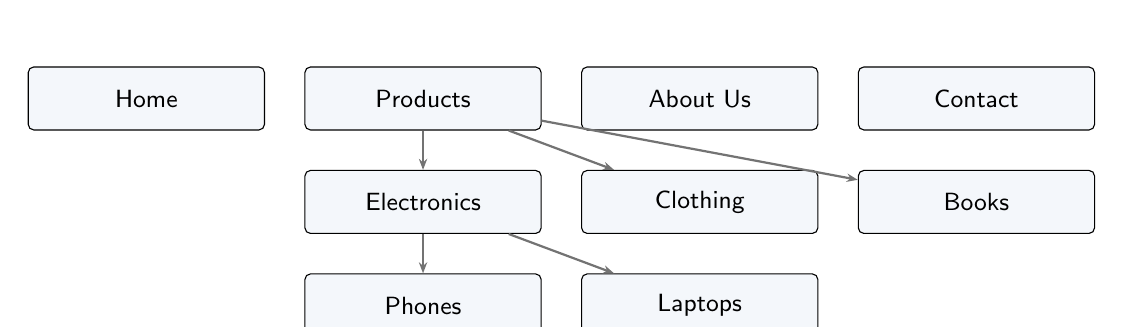
\begin{tikzpicture}[
  node/.style={draw, rounded corners=2pt, minimum width=3.0cm, minimum height=0.8cm, align=center, font=\small\sffamily, fill=nodefill},
  arr/.style={-{Stealth[length=4pt]}, thick, black!55}
]
  \node[node] (home) {Home};
  \node[node, right=0.5cm of home] (products) {Products};
  \node[node, right=0.5cm of products] (about) {About Us};
  \node[node, right=0.5cm of about] (contact) {Contact};

  \node[node, below=0.5cm of products] (electronics) {Electronics};
  \node[node, right=0.5cm of electronics] (clothing) {Clothing};
  \node[node, right=0.5cm of clothing] (books) {Books};

  \node[node, below=0.5cm of electronics] (phones) {Phones};
  \node[node, right=0.5cm of phones] (laptops) {Laptops};

  \draw[arr] (products) -- (electronics);
  \draw[arr] (products) -- (clothing);
  \draw[arr] (products) -- (books);
  \draw[arr] (electronics) -- (phones);
  \draw[arr] (electronics) -- (laptops);
\end{tikzpicture}
\caption{A menu link tree. The \texttt{getLinks()} method recurses
through \texttt{parent\_id} to build this structure. Each level is
a separate \texttt{SELECT * FROM menu\_link WHERE parent\_id = ...}
query (unless cached).}
\label{fig:menu-tree}
\end{figure}

\subsection{The Three Submenu Types}

Each menu link can have one of three submenu types (stored in the
\texttt{property} EAV table under \texttt{group='menu\_link'},
\texttt{key='submenu\_type'}):

\begin{table}[htbp]
\centering
\caption{The three submenu types.}\label{tab:submenu-types}
\small
\begin{tabularx}{\columnwidth}{llX}
\toprule
\textbf{Type} & \textbf{Data source} & \textbf{Rendering} \\
\midrule
\texttt{none} (default) & Children from \texttt{menu\_link} & Recurse into \texttt{getLinks()} for child links. \\
\texttt{page\_id}       & \texttt{property} key \texttt{page\_id} & Embed a CMS page's content as the submenu (calls \texttt{content/page->embed()}). \\
\texttt{html\_content}  & \texttt{description} table & Load localised HTML from the polymorphic \texttt{description} table for this \texttt{menu\_link\_id}. \\
\bottomrule
\end{tabularx}
\end{table}

\subsection{The \texttt{drawLinksGroup()} Method}

The \texttt{drawLinksGroup()} method takes the tree array from
\texttt{getLinks()} and renders it as nested \texttt{<ul>/<li>} HTML.
The exact HTML structure depends on the widget's
\texttt{settings['view']} (which selects the template:
\texttt{links\_main\_menu.tpl}, \texttt{links\_default.tpl},
\texttt{links\_vertical.tpl}, etc.).

\subsection{The Link Templates}

The theme ships 10+ link templates:

\begin{itemize}[leftmargin=1.6em,itemsep=2pt]
  \item \texttt{links\_main\_menu.tpl} --- the main navigation bar.
  \item \texttt{links\_default.tpl} --- a simple \texttt{<ul>} list.
  \item \texttt{links\_vertical.tpl} --- a vertical sidebar menu.
  \item \texttt{links\_overheader.tpl} --- links above the header.
  \item \texttt{links\_01.tpl} through \texttt{links\_07.tpl} ---
        numbered variants for different layout positions.
  \item \texttt{links\_marketo.tpl} --- a marketo-style dropdown.
  \item \texttt{link\_button.tpl} / \texttt{link\_button\_default.tpl}
        --- a single button-style link (used by the separate
        \texttt{link\_button} module).
\end{itemize}

% ============================================================
\section{The Menu Lifecycle Trace}\label{sec:trace}
% ============================================================

\subsection{Admin Creates a Menu}

\begin{enumerate}[leftmargin=1.6em,itemsep=2pt]
  \item Admin navigates to \texttt{?r=content/menu/insert}.
  \item \texttt{ControllerContentMenu::insert()} calls
        \texttt{AdminController::upsert()}.
  \item \texttt{upsert()} validates the form, processes POST data,
        calls \texttt{modelMenu->add(\$data)}.
  \item \texttt{ModelContentMenu::add()} inserts the \texttt{menu} row.
  \item The \texttt{on('save')} hook fires: calls
        \texttt{setItems(\$menu\_id, \$data['link'])}, which inserts
        \texttt{menu\_link} rows (with tree structure via
        \texttt{parent\_id}) and per-link \texttt{property} EAV rows
        (class\_css, submenu\_type, icon, page\_id).
  \item The \texttt{on('save')} hook also writes
        \texttt{object\_to\_store} rows (via the \texttt{relations =
        ["stores"]} declaration) to scope the menu to stores.
  \item Admin activity is logged in \texttt{user\_activity}.
  \item Redirect to \texttt{content/menu} (list view).
\end{enumerate}

\subsection{Storefront Renders the Menu}

\begin{enumerate}[leftmargin=1.6em,itemsep=2pt]
  \item A page loads with a ``links'' widget configured with
        \texttt{menu\_id = 5}.
  \item \texttt{ControllerModuleLinks::init()} registers the
        \texttt{module:settings} filter.
  \item \texttt{ControllerModuleModuleController::index()} calls the
        filter, which calls
        \texttt{drawLinksGroup(getLinks(5))}.
  \item \texttt{getLinks(5, 0)} calls
        \texttt{modelMenu->getAllItems(['menu\_id'=>5,
        'parent\_id'=>0])}.
  \item \texttt{getAllItems()} checks the cache (keyed by
        \texttt{STORE\_ID + language\_id + ...}). On cache miss,
        queries \texttt{SELECT * FROM menu\_link WHERE menu\_id = 5
        AND parent\_id = 0 ORDER BY sort\_order}, then loads
        per-link properties from \texttt{property} and localised
        labels from \texttt{description}.
  \item For each root link, \texttt{getLinks(5, <menu\_link\_id>)}
        is called recursively to fetch children.
  \item For each link with \texttt{submenu\_type = 'page\_id'},
        \texttt{content/page->embed(\$page\_id)} is called to
        embed the page content.
  \item For each link with \texttt{submenu\_type = 'html\_content'},
        \texttt{modelMenu->getDescriptions(\$menu\_link\_id)} is
        called to load the localised HTML.
  \item \texttt{drawLinksGroup()} renders the tree as nested
        \texttt{<ul>/<li>} HTML using the selected template.
  \item The HTML is returned via the \texttt{module:settings} filter
        and stored in \texttt{\$this->data['links']}.
  \item The widget template (\texttt{links\_main\_menu.tpl}) emits
        \texttt{<?php echo \$links; ?>}.
  \item \texttt{Controller::fetch()} substitutes the
        \texttt{\{\%<widget\_name>\%\}} placeholder with the rendered
        HTML (v3's composite-view pattern).
\end{enumerate}

% ============================================================
\section{Cross-Cutting Findings}\label{sec:findings}
% ============================================================

\subsection{The Menu System Exercises Every Cross-Cutting Pattern}

The menu system is a microcosm of the Necoyoad architecture:

\begin{itemize}[leftmargin=1.6em,itemsep=2pt]
  \item \textbf{AdminController declarative CRUD} (v6): the menu
        controller is 495 lines, but most of that is the
        \texttt{grid:data} filter and form customisation. The actual
        CRUD is inherited from AdminController.
  \item \textbf{Polymorphic \texttt{description} table} (v5):
        menu links use \texttt{object\_type = 'menu\_link'} for
        localised labels and HTML submenu content.
  \item \textbf{EAV \texttt{property} table} (v3, v5): per-link
        metadata (CSS class, submenu type, icon, page ID) stored as
        key-value pairs under \texttt{group = 'menu\_link'}.
  \item \textbf{\texttt{object\_to\_store} junction} (v5): menus are
        scoped to stores via the \texttt{relations = ["stores"]}
        declaration.
  \item \textbf{Widget rendering pipeline} (v3): the links widget
        extends \texttt{ControllerModuleModuleController} and uses
        the \texttt{module:settings} filter to inject the rendered
        menu tree.
  \item \textbf{Multi-store/multi-language} (v5): the storefront
        cache key includes \texttt{STORE\_ID} and
        \texttt{config\_language\_id}, so each (store, language)
        pair has its own cached menu tree.
\end{itemize}

\subsection{The Recursive Tree Rendering is N+1 Query Prone}

\begin{findingbox}[N+1 query pattern in tree rendering]
The \texttt{getLinks()} method recurses through the tree by calling
\texttt{getAllItems()} for each parent. Each call is a separate
\texttt{SELECT * FROM menu\_link WHERE parent\_id = ...} query,
plus per-link \texttt{property} and \texttt{description} lookups.
For a 3-level menu with 5 root items, 3 children each, and 2
grandchildren each, this is $1 + 5 + 15 = 21$ queries for the
tree, plus $21 \times 2 = 42$ property/description queries --- 63
queries total.

The cache (keyed by store + language + data) absorbs this on
subsequent requests, but the first request (or any request after
a cache clear) pays the full N+1 cost.
\end{findingbox}

\subsection{The \texttt{var\_dump} Left in Production Code}

\begin{findingbox}[\texttt{var\_dump()} in the links widget]
The \texttt{ControllerModuleLinks::getLinks()} method contains a
\texttt{var\_dump(\$descriptions)} call (line 82) that fires when
\texttt{submenu\_type === 'html\_content'}. This is debug code
left in production. Every menu link with an HTML-content submenu
type will dump the descriptions array to the browser before the
menu HTML.
\end{findingbox}

\subsection{The Menu Link Label is Both in \texttt{menu\_link.tag} and \texttt{description.title}}

The \texttt{menu\_link} table has a \texttt{tag} column (the visible
label), but the polymorphic \texttt{description} table also has a
\texttt{title} column for localised labels. The storefront model
loads both. If a localised description exists, it presumably
overrides the \texttt{tag}; if not, the \texttt{tag} is used. This
dual storage (non-localised \texttt{tag} + localised
\texttt{description.title}) is the same pattern used by products
(\texttt{product.model} + \texttt{description.title}).

% ============================================================
\section{Closing Observations}\label{sec:observations}
% ============================================================

\subsection{The Menu System is a Clean Application of the Architecture}

The menu system is one of the cleanest applications of the Necoyoad
architecture. The admin controller is almost entirely declarative
(via AdminController), the model uses the standard
\texttt{on('save')}/\texttt{on('delete')} hook pattern, the
storefront model uses the standard cache pattern, and the widget
module uses the standard \texttt{module:settings} filter pattern.
No special cases, no custom SQL (beyond the model's declarative
fields), no custom rendering logic (beyond the recursive tree).

\subsection{The Menu System is Where the Patterns Compose}

The menu system is where all the cross-cutting patterns compose:
AdminController (v6) for CRUD, polymorphic description (v5) for
localisation, EAV property (v3, v5) for metadata,
object\_to\_store (v5) for multi-store, widget rendering (v3) for
display, and multi-language caching (v5) for performance. v7 is
the volume that ties them all together in a single subsystem.

\subsection{Final Note}

v7 confirms that the Necoyoad menu system is a clean, recursive,
multi-store, multi-language navigation system built on the
platform's cross-cutting patterns. The AdminController declarative
CRUD, the polymorphic description table, the EAV property table, and
the widget rendering pipeline all work together to produce a menu
system that is both flexible (tree structure, three submenu types,
per-link CSS/icon) and consistent with the rest of the platform.

\appendix
\section{Glossary}\label{app:glossary}
\begin{table}[htbp]
\centering
\caption{Glossary of menu system terms.}\label{tab:glossary-v7}
\footnotesize\sloppy
\begin{tabularx}{\columnwidth}{>{\raggedright\arraybackslash}p{3.5cm}X}
\toprule
\textbf{Term} & \textbf{Meaning} \\
\midrule
Menu & A named collection of links, scoped to a store and position. \\
Menu link & A single link within a menu, with tree structure via \texttt{parent\_id}. \\
Submenu type & The \texttt{property} EAV key that controls how a link's submenu is rendered: \texttt{none} (children), \texttt{page\_id} (embedded CMS page), or \texttt{html\_content} (localised HTML). \\
Links widget & The storefront module (\texttt{ControllerModuleLinks}) that renders a menu tree recursively. \\
\texttt{drawLinksGroup()} & The method that converts the tree array into nested \texttt{<ul>/<li>} HTML. \\
\texttt{getLinks()} & The recursive method that fetches menu links from the model and builds the tree array. \\
\bottomrule
\end{tabularx}
\end{table}
\end{document}
